% Appendix: DM-ratio sensitivity v5.2
\section*{Appendix: DM-ratio sensitivity (v5.2)}
\addcontentsline{toc}{section}{Appendix: DM-ratio sensitivity (v5.2)}
\label{appendix:dm-ratio-v5.2}

This appendix summarizes the results of the DM-ratio sensitivity analysis (v5.2).
The analysis compares the L-ToEC prediction R = 5 + e^{-\lambda} under Poisson sampling and
alternative rate models (negative binomial, log-normal mixtures), and compares the prediction
at \(\lambda=1\) to Planck 2018 values.

\paragraph{Summary:}
Using the Planck-derived values \(\Omega_c h^2 = 0.1200\) and \(\Omega_b h^2 = 0.02237\),
we obtain an observed ratio \(\Omega_c/\Omega_b \approx 5.36433\).
The L-ToEC Poisson-based prediction at \(\lambda=1\) is
\(R = 5 + e^{-1} \approx 5.36788\), giving an absolute error of approximately 0.00355
(\(~0.066\%\) relative).

\paragraph{Figures:}
The following figures were generated by a reproducible script (docs/physics/specs/dm_ratio_v5.2_run.py).

\begin{figure}[h]
  \centering
  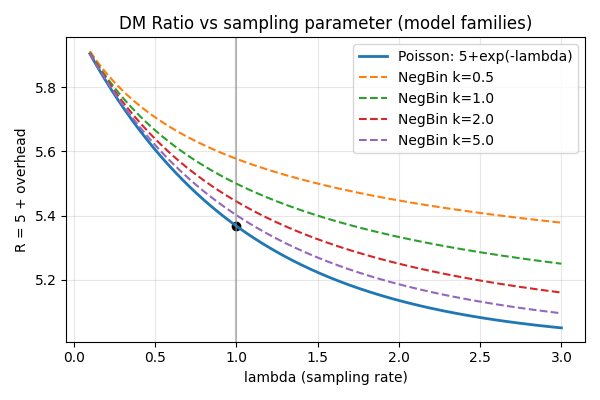
\includegraphics[width=0.8\textwidth]{notebooks/dm_ratio_lambda_plot.png}
  \caption{DM ratio vs sampling parameter for Poisson and negative-binomial families.}
  \label{fig:dm_ratio_lambda}
\end{figure}

\begin{figure}[h]
  \centering
  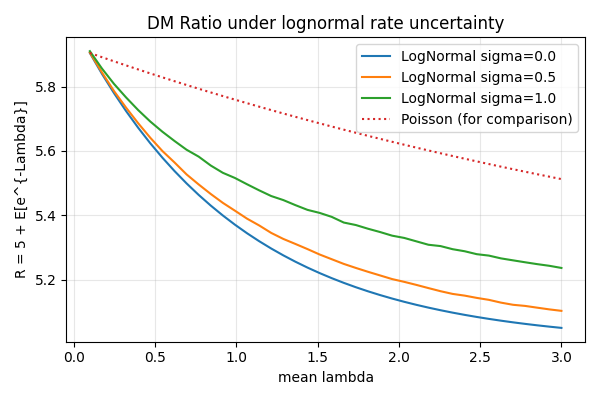
\includegraphics[width=0.8\textwidth]{notebooks/dm_ratio_lognorm_plot.png}
  \caption{DM ratio under log-normal rate uncertainty (mixture models).}
  \label{fig:dm_ratio_lognorm}
\end{figure}

\paragraph{Reproducibility:}
Full artifacts are available in the repository:
\begin{itemize}
  \item Script: \texttt{docs/physics/specs/dm_ratio_v5.2_run.py}
  \item Report: \texttt{docs/physics/notebooks/dm_ratio_sensitivity_report.txt}
  \item PDF: \texttt{docs/physics/notebooks/dm_ratio_sensitivity_v5.2.pdf}
\end{itemize}

\paragraph{Interpretation:}
The Poisson-based prediction closely matches the Planck value within \(\mathcal{O}(10^{-3})\).
Alternative rate models (overdispersion, heavy-tailed uncertainty) produce deviations of order
\(10^{-3}\) to \(10^{-2}\) depending on parameter choices; see the reproducible script for details.

